\documentclass[border=5pt]{standalone}

\usepackage{tikz}

\usetikzlibrary{calc}

\newcommand*{\base}{0.5cm}
\newcommand*{\bs}{6*\base}
\newcommand*{\dx}{0.1cm}%

\tikzset{
	place/.style={
    	circle,
	    minimum size =1.5*\base,
    	draw=black,
	    fill=white,
    	thick,
		outer sep=0.5*\base
	},
	background/.style={
		circle,
    	minimum size =2*\base,
	    draw=white,
    	fill=black,
    	very thick,
		outer sep=0.5*\base
	},
	bbox/.style n args={3}{
		minimum size = \bs,
    	draw = #1,
    	very thick,
		fill = #2,
		fill opacity = #3,
		}
	}
	
\begin{document}
    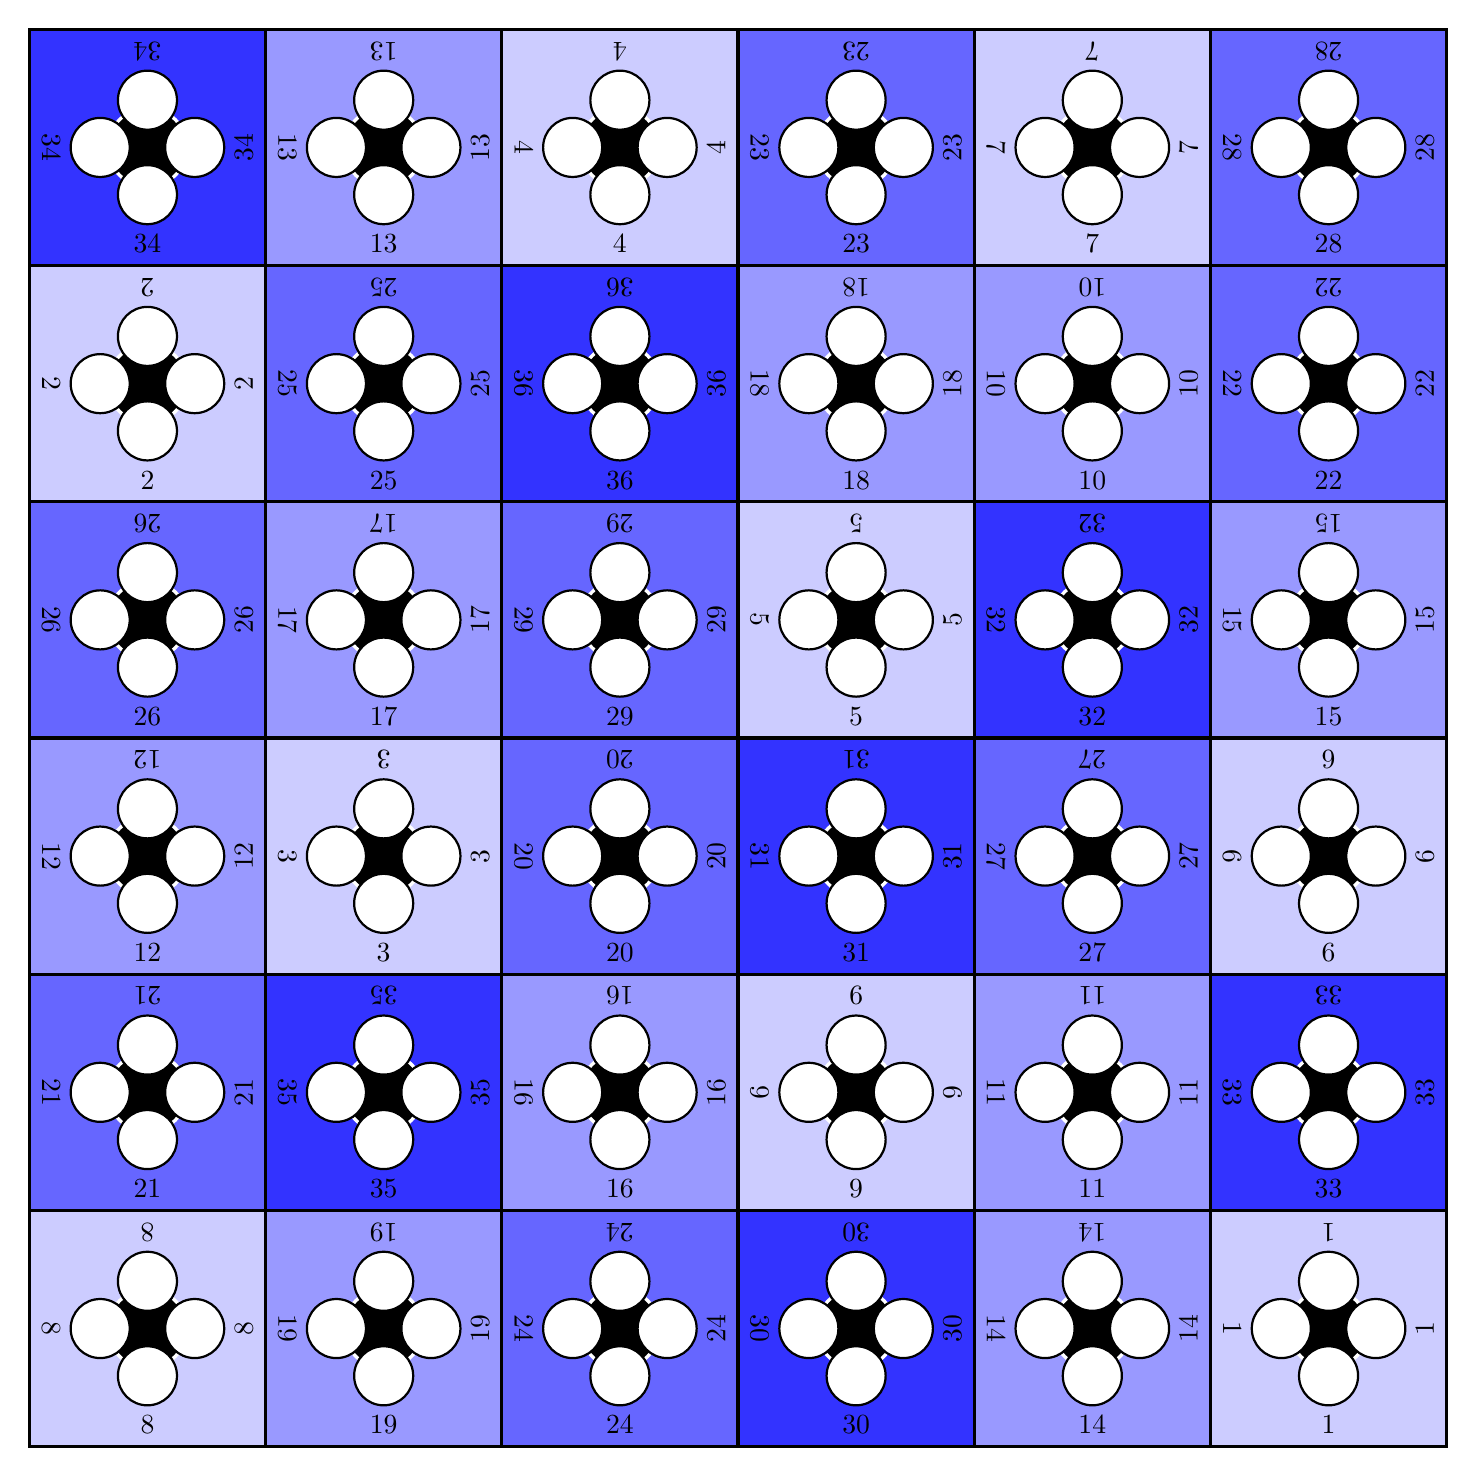
\begin{tikzpicture}
    	\def\nums{%
    	    { 8,19,24,30,14, 1,%
			 21,35,16, 9,11,33,%
			 12, 3,20,31,27, 6,%
			 26,17,29, 5,32,15,%
			  2,25,36,18,10,22,%
			 34,13, 4,23, 7,28 %
			}};
    	\foreach \x in {0,...,5} {
    		\foreach \y in {0,...,5} {
    			\node (sq) [bbox={black}{blue}{floor((\nums[\x+6*\y]/10))*0.2+0.2}] at (\x*\bs,\y*\bs) {};
        		\node (cc) [background] at (\x*\bs,\y*\bs) {};
        		\node (ce\x\y) [place] at (\x*\bs+\base+\dx,\y*\bs) {};
        		\node (cn\x\y) [place] at (\x*\bs,\y*\bs+\base+\dx) {};
        		\node (cw\x\y) [place] at (\x*\bs-\base-\dx,\y*\bs) {};
        		\node (cs\x\y) [place] at (\x*\bs,\y*\bs-\base-\dx) {};
        		{\pgfmathparse{\nums[\x+6*\y]};
        		\node[rotate=90] at (ce\x\y.east) {\pgfmathresult};
        		\node[rotate=180] at (cn\x\y.north) {\pgfmathresult};
        		\node[rotate=-90] at (cw\x\y.west) {\pgfmathresult};
        		\node at (cs\x\y.south) {\pgfmathresult};
        		}
        	};
        };
    \end{tikzpicture}
\end{document}